\documentclass[12pt]{article}
\usepackage[slovene]{babel}
\usepackage[utf8]{inputenc}
\usepackage[T2A]{fontenc}
\usepackage{amsmath}
\usepackage{amsfonts}
\usepackage{amssymb}
\usepackage[version=4]{mhchem}
\usepackage{stmaryrd}
\usepackage{graphicx}
\usepackage[export]{adjustbox}
\graphicspath{ {./images/} }
\usepackage{physics}
\usepackage{geometry}
\geometry{left=2cm,right=2cm,top=2cm,bottom=2cm}



\title{\textbf{Ultra zvok}}
\author{Samo Krejan}
\date{marec 2025}


\begin{document}
\maketitle

\section{Uvod}

Ultrazvok, kot vse nedestruktivne metode opazovanja sloni na pojavih absorbcije, sipanja in odboja valovanja v notranjosti telesa. Relavanten parameter je valovna dolžina uporabljeega valovanja, ki nam določa ločljivost, hkrati pa mora biti tudi absorbcija in sipanje zmerno. Poleg tega potrebujemo primerne vire in detektorje valovanja (ultrazvoka).

Seveda se ultrazvok že dolgo uporablja v medicini, poleg tega pa je zelo uporaben tudi v kovinski industriji za zaznavanje nečistoč v npr.: blokih železa. Ultrazvok s frekvenco nekaj $MHz$ ima v večini snovi valovno dolžino okoli milimetra, kar zadostuje za opazovanje človeškega telesa ter za analizo jeklenih blokov. Merjenje jakosti odbojev ultrazvoka v različnih globinah merjenca je najbolj pogost način meritve. V tem primeru merimo čas, ki ga valovanje porabi od izvora do nehomogenosti, ki valovanje delno odbija, in nazaj do detektorja. Meritev časa nam omogoča pošiljanje sunkov ultrazvočnega valovanja, s čimer je taka priprava močno podobna radarju. Za izvor uporabimo kar piezo kristal, ki odda le kratek sunek, dolg nekaj valovnih dolžin, nato pa meri jakost odbitega signala v odvisnosti od časa. Isti piezokristal lahko uporabimo tudi kot sprejemnik valovanaj, s čemer dobimo eno-dimenzionalni prerez opazovanega telesa. Če uporabimo večje število izvorov in detektojev (npr.: 256) lahko dobimo dvo-dimenzionalni presek. To uporabljajo na primer v ginekologiji.

Moderne ultrazvočne priprave omogočajo tudi merjenje premikov frekvence kot posledico Dopllerjevega pojava, s čimer lahko analiziramo tudi premikanje teles (nehomogenosti). Seveda uporabljajo tudi drugačne metode.

Za nas zanimivo je tudi določanje hitrosti ultrazvoka v snovi saj je le-ta povezana z različnimi lastnostmi snovi. V homogenih snoveh lahko tako na primer določimo prožni modul $E$, strižni modul $G$ in pa Poissonovo število $\mu$. Velikrat smo recimo že videli s kakšno hitrostjo $c$ se širi vaovanje po tanki palici z gostoto $\rho$ (\ref{tanka}):

\begin{equation}
    c^{2} = \frac{E}{\rho}
    \label{tanka}
\end{equation}
V razsežnem sredstvu je stvar nekoliko drugačna. Hitrost širjenja valovanja namreč opiše enačba (\ref{razsežna})

\begin{equation}
    c^{2} = \frac{E(1-\mu)}{\rho(1+\mu)(1-2\mu)}
    \label{razsežna}
\end{equation}
Obe ti enačbi veljata le za longitudinalno valovanje. Pri transferzalnem je zadeva še nekoliko drugačna, saj je tam vseskupaj odvisno bolj od strižnega modula. Enačba za hitrost tam torej izgleda kot (\ref{trans}).

\begin{equation}
    c^2 = \frac{G}{\rho} = \frac{E}{2\rho(1+\mu)}
    \label{trans}
\end{equation}

Hitrost transferzalnega valovanja v tanki palici, je še bolj zakomplicirana, a se z njo tu ne bomo ukvarjali.

\section{Potrebščine}

\begin{itemize}
    \item Ultrazvočni defektoskop kot izvor in detektor valovanja,
    \item digitalni osciloskop za opazovanje signala (SigLent SDM 3065X), USB ključek,
    \item ultrazvočna sonda za longitudinalno valovanje MB4S-N z resonančno frekvenco 4 MHz (proizvajalec GE Kreutkramer) in za transverzalno valovanje V155 z resonančno frekvenco 5 MHz (proizvajalec Panamatrics),
    \item posoda z vodo s sondo MB4S-N in z nastavljivo odmevno površino, atenuator (dušilec) signala,
    \item standardni miniaturni in kalibracijski blok normalne velikosti nepravilnih oblik z režami in izvrtinami, (slika \ref{blok})
    \item valji iz jekla, aluminija in drugih materialov,
    \item kontaktne paste za zapolnitev reže med sondami in merjenci,
    \item stojalo za montažo sonde in valjastih merjencev, BNC kabli.
\end{itemize}

\begin{figure}[h]
\begin{center}
    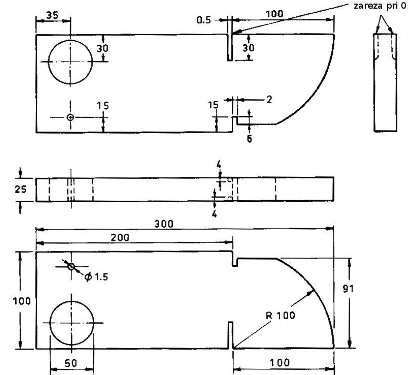
\includegraphics[width=7cm]{blok.png}
    \caption{kalibracijski blok}
    \label{blok}
\end{center}
\end{figure}

\section{Naloga}

\begin{itemize}
    \item Opazujte odboj longitudinalnega ultrazvočnega valovanja na različnih ploskvah priloženega merjenca nepravilnih oblik z izvrtinami in zarezami. Kalibrirajte skalo na zaslonu osciloskopa v mm poti valovanja v jeklu.
    \item Poiščite odboj na izvrtini premera 1mm in določi njen položaj glede na zunanje ploskve merjenca. Oceni globinsko ostrino meritve.
    \item Določite hitrost longitudinalnega in transverzalnega ultrazvočnega valovanja v jeklu in aluminiju, ali v drugem materialu. Uporabi ultrazvočni interferometer. Izračunajte prožnostni modul $E$, strižni modul $G$ in Poissonovo število $\mu$.
\end{itemize}

\section{Rezultati in analiza}

Najprej smo izmerili daljšo in krajšo višino kalibracijskega bloka: $h = 10,020 \pm 0,002\ cm$ in $h' = 9,118\pm 0,002\ cm$. Z ultrazvokom smo izmerili čas med prvim in drugim odbojem. Čas prevega in drugega odboja, razlika v časih in preračunana hitrost zvoka v jeklu so podani v tabeli \ref{blok-tabela}. Hitrost valovanja je izračunana kot $c = \frac{\Delta t}{2h}$ saj signal potuje v obe smeri.
\bigskip
kle pride tabela type shi
\bigskip

Za tem smo opazovali odboj ultra zvoka na tanki zarezi. Signal, ki smo ga prejeli je prikazan na grafu \ref{reža}. Iz grafa odčitamo po dva odboja za tri različne signale: na večji širina, na manjši širini in na reži. Časi signalov so v tabeli \ref{reža-tabela}



\end{document}